% 
% Annual Cognitive Science Conference
% Sample LaTeX Paper -- Proceedings Format
% 

% Original : Ashwin Ram (ashwin@cc.gatech.edu)       04/01/1994
% Modified : Johanna Moore (jmoore@cs.pitt.edu)      03/17/1995
% Modified : David Noelle (noelle@ucsd.edu)          03/15/1996
% Modified : Pat Langley (langley@cs.stanford.edu)   01/26/1997
% Latex2e corrections by Ramin Charles Nakisa        01/28/1997 
% Modified : Tina Eliassi-Rad (eliassi@cs.wisc.edu)  01/31/1998
% Modified : Trisha Yannuzzi (trisha@ircs.upenn.edu) 12/28/1999 (in process)
% Modified : Mary Ellen Foster (M.E.Foster@ed.ac.uk) 12/11/2000
% Modified : Ken Forbus                              01/23/2004
% Modified : Eli M. Silk (esilk@pitt.edu)            05/24/2005
% Modified: Niels Taatgen (taatgen@cmu.edu) 10/24/2006

%% Change ``a4paper'' in the following line to ``letterpaper'' if you are
%% producing a letter-format document.

\documentclass[10pt,letterpaper]{article}

\usepackage{cogsci}
\usepackage{pslatex}
\usepackage{apacite}

\title{Modeling the dynamics of classroom education using teaching games}
 
\author{{\large \bf Morton Ann Gernsbacher (MAG@Macc.Wisc.Edu)} \\
  Department of Psychology, 1202 W. Johnson Street \\
  Madison, WI 53706 USA}


\begin{document}

\maketitle


\begin{abstract}
We describe a model of classroom teaching that construes teaching as communication to a heterogeneous audience. A number of basic educational results fall out of this construal, including (1) decreasing mean performance with the increasing size and variability among students in a class, (2) increases in performance based on grouping students by abilities, and (3) the value of formative evaluation to enhance teachers' knowledge of student ability.

\textbf{Keywords:} 
Add your choice of indexing terms or keywords; kindly use a semi-colon; between each term.
\end{abstract}


\section{Introduction}

To fill this need, we describe a model of classroom teaching. This model captures phenomena that have to do with the informational dynamics of the classroom---how much information can be transferred between a teacher and a group of students with certain abilities and prior beliefs. It has nothing to say about another---perhaps ultimately more important---part of the classroom experience, its motivational dynamics.  

What are the functions of such a model? 

\section{Teaching games}

The basic unit of our analysis is a teaching game. In such a game, teacher $T$ attempts to provide information to students $S = {s_1 ... s_m}$. Teacher conveys information by choosing examples $E = {e_1 ... e_n}$ to illustrate an underlying concept $C$, based on some estimate of the students' prior knowledge and abilities $\hat{S} = {\hat{s_1} ... \hat{s_m}}$. Learners in turn attempt to recover $C$ with maximal fidelity. The teacher's payoff is determined by a test, administered to each of the learners, with some payoff function. 

We will begin by considering a very simple form of this sort of game, with only one student, one example, and perfect teacher knowledge of that student's abilities. We think of this as the ``optimal tutoring'' regime. In this simple game, the concept to be learned is the parameter on a Bernoulli variable (the weight on a coin, e.g.). The teacher must choose a single observation to give to the student. 

\subsection{Students}

\begin{figure}[t]
\begin{center}
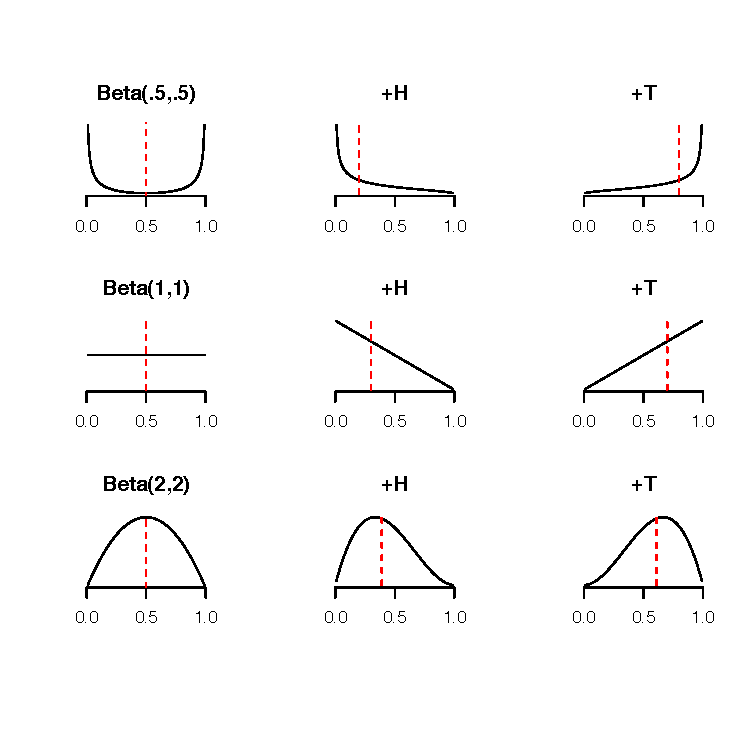
\includegraphics[width=5.5in]{figures/students.pdf}
\end{center}
\caption{\label{fig:students} Examples of the beta-bernoulli distribution with different priors and patterns of evidence. Black curves show probability distribution with a given prior (left column) and after observing a single tail or head (middle and right columns). Red lines show posterior mean.}
\end{figure}

We model the student here as a Bayesian (optimal) estimator of this Bernoulli distribution, using a conjugate Beta-Bernoulli distribution. This model is very convenient: the form of the prior distribution is $Beta(\alpha,\beta)$, and the form of the posterior can be written $Beta(\alpha+t,\beta+h)$ where $t$ and $h$ represent the number of heads (0) and tails (t) observed in the data respectively. In this sense, if $t$ and $h$ are the \emph{counts} of observed data, then $\alpha$ and $\beta$ can be referred to as \emph{pseudo-counts}.

This formulation also gives us a way to model both the student's abilities and their prior knowledge about the situation. Consider the example beta-Bernoulli distributions shown in Figure \ref{fig:students}. Symmetric priors of $\alpha=\beta=.5$ lead to a bias that the target coin weight is either 0 or 1, while $\alpha=\beta=.5$ leads to a bias towards fairer coins. As the strength of the prior grows, the effect of observing a single coin flip becomes weaker. 

Under this formulation, the prior controls both the speed at which a student will learn and their overall bias. For example, as $\alpha$ and $\beta$ both go towards 0, the student's estimate converges to a maximum-likelihood estimate based on the observed data alone. In contrast, as $\alpha$ and $\beta$ both get larger, the student makes less and less use of the data and is more and more reliant on the shape of the prior distribution. The relative weights of $\alpha$ and $\beta$ control the student's bias---greater pseudo-counts on one or the other will lead to greater bias to believe that the correct parameter is lower or higher. We explore each of these scenarios---learning speed and bias---below.

\begin{equation}
P(S = c) = \frac{C^{\alpha-1}(1-C)^{\beta-1}}{B(\alpha,\beta)} 
\end{equation}

where $B$ is the beta function, and hence

\begin{equation}
P(S' = C)  = \frac{C^{\alpha+h-1}(1-C)^{\beta+t-1}}{B(\alpha+h,\beta-t)} 
\end{equation}

\subsection{Evaluation}

% We define two different metrics of student progress. The first is derived from the idea of administering ``tests'' to a student and evaluating their outcome on that test. The second is based on the idea of measuring the amount of information (in bits) that has been conveyed by the teacher, given the student's initial state. We describe each of these in turn. 

% \subsubsection{Testing-based evaluation}

\begin{figure}[t]
\begin{center}
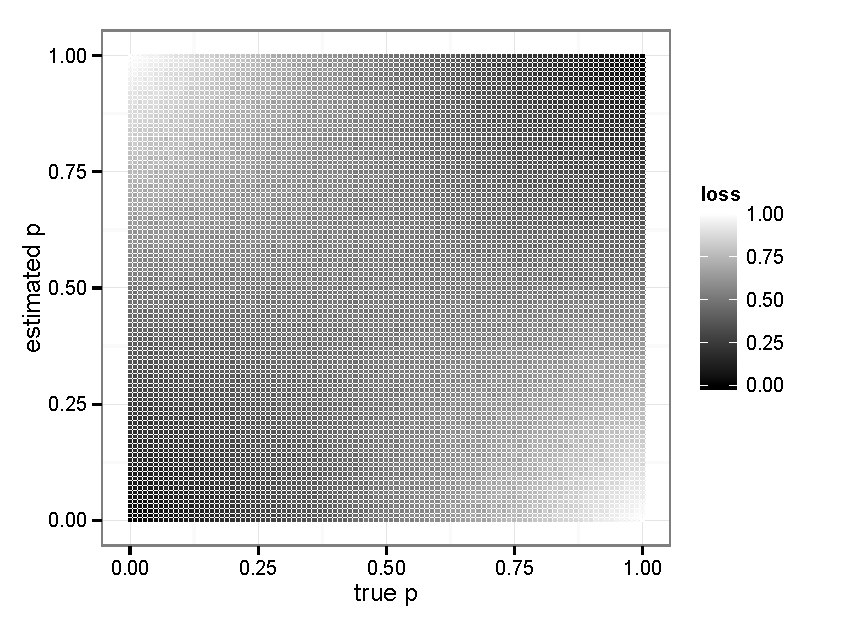
\includegraphics[width=5.5in]{figures/loss1.pdf}
\end{center}
\caption{\label{fig:loss1} Map of the loss function for testing-based evaluation, assessed numerically.}
\end{figure}

We define a test as a set of examples drawn randomly from $c$ that must be guessed. 

\begin{eqnarray}
L(S',C) &=& P(S' = C) \\
&=&
\end{eqnarray}

% \subsubsection{Information-theoretic evaluation}

% We are also interested in the total information gain for a student (and for a class) based on some instructional choices. For example, if $C=.9$ and a student begins as $Beta(2,2)$ and is instructed with $H$, $H$, $H$, she will update to $Beta(2,5)$. Her information gain is thus the Kullback-Leibler divergence $D_{KL} (Beta(2,5) || Beta(2,2))$. 


% More generally, this can be written:

% \begin{eqnarray}
% D_{KL} (S' || S) &=& \int_{-\infty}^{\infty} {ln (\frac{Beta(\alpha+t,\beta+h)}{Beta(\alpha,\beta)}) Beta(\alpha+t,\beta+h) d\alpha d\beta}
% \end{eqnarray}

\subsection{Teachers}

\section{Simulations}

\subsection{Classroom size}

\subsection{Tracking}

\subsection{Testing for better knowledge}

\section{Decision-theoretic analyses}


\section{Acknowledgments}

Place acknowledgments (including funding information) in a section at
the end of the paper.


\section{References Instructions}

Follow the APA Publication Manual for citation format, both within the
text and in the reference list, with the following exceptions: (a) do
not cite the page numbers of any book, including chapters in edited
volumes; (b) use the same format for unpublished references as for
published ones. Alphabetize references by the surnames of the authors,
with single author entries preceding multiple author entries. Order
references by the same authors by the year of publication, with the
earliest first.

Use a first level section heading for the reference list. Use a
hanging indent style, with the first line of the reference flush
against the left margin and subsequent lines indented by 1/8~inch.
Below are example references for a conference paper, book chapter,
journal article, technical report, dissertation, book, and edited
volume, respectively.

\nocite{ChalnickBillman1988a}
\nocite{Feigenbaum1963a}
\nocite{Hill1983a}
\nocite{OhlssonLangley1985a}
\nocite{Lewis1978a}
\nocite{NewellSimon1972a}
\nocite{ShragerLangley1990a}


\bibliographystyle{apacite}

\setlength{\bibleftmargin}{.125in}
\setlength{\bibindent}{-\bibleftmargin}

\bibliography{CogSci_Template}


\end{document}
